\documentclass[tikz,border=10pt]{standalone}
\usetikzlibrary{arrows.meta, positioning, calc}

\begin{document}

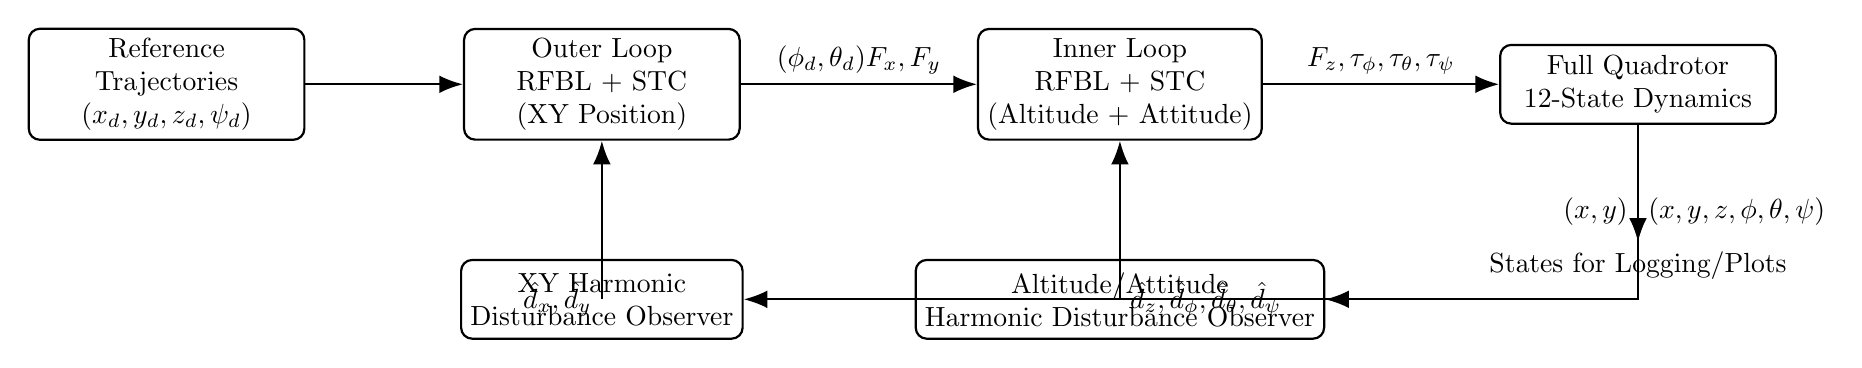
\begin{tikzpicture}[
    block/.style = {rectangle, draw, thick, rounded corners,
                    align=center, minimum width=3.5cm, minimum height=1cm},
    sum/.style   = {circle, draw, inner sep=1pt},
    arrow/.style = {thick, -{Latex[length=3mm]}}
]

% =====================
% Nodes (left to right)
% =====================

% References
\node[block] (ref) {Reference\\ Trajectories\\ $(x_d,y_d,z_d,\psi_d)$};

% Outer loop controller
\node[block, right=2cm of ref] (outer) {Outer Loop\\ RFBL + STC\\ (XY Position)};

% Inner loop controller
\node[block, right=3cm of outer] (inner) {Inner Loop\\ RFBL + STC\\ (Altitude + Attitude)};

% Disturbance Observers
\node[block, below=1.5cm of outer] (do_xy) {XY Harmonic\\ Disturbance Observer};
\node[block, below=1.5cm of inner] (do_att) {Altitude/Attitude\\ Harmonic Disturbance Observer};

% Dynamics
\node[block, right=3cm of inner] (dyn) {Full Quadrotor\\ 12-State Dynamics};

% ====================================
% Connections (control flow)
% ====================================

\draw[arrow] (ref) -- (outer);

\draw[arrow] (outer) -- node[midway,above]{$(\phi_d,\theta_d)$\\$F_x,F_y$} (inner);

\draw[arrow] (inner) -- node[midway,above]{$F_z,\tau_\phi,\tau_\theta,\tau_\psi$} (dyn);

\draw[arrow] (dyn) |- node[pos=0.25,right]{$(x,y,z,\phi,\theta,\psi)$} (do_att);
\draw[arrow] (dyn) |- node[pos=0.25,left]{$(x,y)$} (do_xy);

\draw[arrow] (do_att) -| node[pos=0.25,right]{$\hat d_z,\hat d_\phi,\hat d_\theta,\hat d_\psi$} (inner);
\draw[arrow] (do_xy) -| node[pos=0.25,left]{$\hat d_x,\hat d_y$} (outer);

% Output back to reference/monitoring
\draw[arrow] (dyn) -- ++(0,-2) node[below]{States for Logging/Plots};

\end{tikzpicture}

\end{document}
